% -------------------- Packages --------------------

\documentclass{assignment}[2019/10/15]
\usepackage[lineno]{packages}[2019/11/14]

\usepackage[linesnumbered, lined, ruled, commentsnumbered]{algorithm2e}
\labelformat{algocf}{Algorithm #1}

% -------------------- Settings --------------------

% Title

\title{Report for Iterative Methods: Jacobi, G-S, Multigrid}
\author{Chen Xuyang}
\date{\today}
\institute{School of Mathematical Science}
\professor{Chen Suqin}
\course{Numerical Partial Differential Equations}
\subject{Numerical Partial Differential Equations}
\keywords{}

% -------------------- New commands --------------------

\newcommand{\BR}{\symbb{R}}
\newcommand{\BZ}{\symbb{Z}}
\newcommand{\diag}{\mathop{}\!\symup{diag}}
\newcommand{\pr}{\mathop{}\!\symup{Pr}}
\newcommand{\expect}{\mathop{}\!\symup{E}}
\newcommand{\cov}{\mathop{}\!\symup{Cov}}
\newcommand{\var}{\mathop{}\!\symup{Var}}

\def\multiset#1#2{\ensuremath{\left(\kern-.3em\left(\genfrac{}{}{0pt}{}{#1}{#2}\right)\kern-.3em\right)}}

\newcommand{\lr}[3]{\left#1#3\right#2}
\newcommand{\lmr}[5]{\left#1#4\middle#2#5\right#3}

% -------------------- Document --------------------

\begin{document}
    \maketitle
    \tableofcontents
    \clearpage

    \section{Background}

    Omitted.

    \section{Questions}

    The default for these questions is a $24\times 24$ grid unless otherwise specified.

    \begin{enumerate}[1)]
        \item Write down the Jacobi and the Gauss-Seidel iteration schemes to solve the above Poisson's equation and draw a block diagram or pseudo code outlining your proposed implementation.
        \item Code the Jacobi and G-S routines. Allow variable specification of the ``fineness" of the grid (values such as, $6\times 6, 12\times 12, 24\times 24$, etc). Note: For simplicity we shall assume that for the source blocks all nodes, including the block boundaries, have $f=1$. Also, for two adjacent source blocks, the points on the common boundary also have $f=1$.
        \begin{enumerate}[a.]
            \item Implement a relaxation scheme for both.
            \item Show the convergence of you Jacobi and G-S solver for the above arrangement of blocks (1, 7, 14, 16), with various relaxation factors. What is the optimal relaxation factor for the G-S method?
            \item A sample solution for the example case (1, 7, 14, 16) is provided in Table 1 (left). Verify that your solver produces a similar output.
        \end{enumerate}
        {\bf Hint}: For later problems it will be convenient to construct a function that takes an input including the 4 numbers corresponding to the test blocks ($\symup{B1, B2, B3, B4} \in 1-16$), and returns the normal derivative around the perimeter as an output.
        \item Implement a multigrid routine that will perform a two-grid method. Show and explain the restriction and prolongation method you choose to implement. Try a relaxation factor of $1/2$ and $4/5$.
        \begin{enumerate}[a.]
            \item Compare the convergence of the multigrid routine with the various other methods. Which method is best? Which relaxation factor for your multigrid routine is better, $1/2$ or $4/5$?
            \item Implement a $(1, 2, 1)$ and a $(2, 4, 2)$ (fine, coarse, fine), routine for the multigrid. How do the routines compare?
        \end{enumerate}
        \item Using the best method (based on convergence rate), and the given normal flux distribution, determine the unknown positions of the four blocks, for the $\mathop{}\!\symup{\partial}\phi/\mathop{}\!\symup{\partial}n=g(x)$ given in Table 1 (right). Pictorially show where the sources are located.
        \item {\bf BONUS}: Write a generalized V-cycle multigrid routine which allows multiple grid refinements. Show convergence for the 2, 3 and 4 grid refinement V-cycles. How do they compare to the other iterative routines?
    \end{enumerate}

    \section{Notations}

    Assume we use an $n\times n$ grid to discretize a pde problem. Let $(x_i, y_j)^T = (i/n, j/n)^T$ be a point in closed unit square, where $0\leq i, j\leq n$. Let $f$ be any function defined on the closed unit square. Then we shall denote its value on a grid point, say $f(x_i, y_j)$, by $f_{i, j}$.

    All programs are tested in a PC with AMD Ryzen 5 3500X 6-Core Processor 3.59 GHZ, 16.0 GB RAM, Windows 10 Pro 1919 64-bit operating system and MATLAB R2020a x64 application.

    \section{Pseudo Code for Jacobi and G-S Iteration Schemes}

    We are to solve the Poisson's equation
    \begin{equation}
        \begin{cases}
            -\mathop{}\!\symup{\nabla}^2 \phi(x, y) = f(x, y), & (x, y)\in D,\\
            \phi(x, y) = 0, &(x, y)\in \mathop{}\!\symup{\partial} D,
        \end{cases}
    \end{equation}
    where $D$ denotes the open unit square. Discretize the problem using an $n\times n$ grid, then we will obtain the linear equations
    \begin{equation}
        \begin{cases}
            \phi_{i, j} = 0, &ij=0,\\
            n^2\left(4\phi_{i, j}-\phi_{i-1, j}-\phi_{i, j-1}-\phi_{i+1,j}-\phi_{i,j+1}\right)=f_{i, j}, &ij\neq 0.
        \end{cases}
    \end{equation}

    Jacobi (see \ref{algo: Jacobi}) and Gauss-Seidel (see \ref{algo: G-S}) iteration schemes differ in the way of deriving the value of the $(r+1)$-th iteration $\phi_{i, j}^r$ by the computed values. Jacobi iteration scheme only uses those values computed in the $r$-th iteration, while G-S iteration scheme updates some old values which is computed in the current iteration.

    \begin{algorithm}[htb]
        \caption{Jacobi Iteration Scheme}
        \label{algo: Jacobi}

        \KwIn{A force matrix $f$ of size $(n+1)\times (n+1)$, a relaxation parameter $\omega$ with $0<\omega<1$, an initial guess matrix $\phi^0$ of the unknowns of size $(n+1)\times(n+1)$ and a small positive number $\epsilon$ which decides when to end the algorithm}
        \KwOut{A matrix of the unknowns $\phi$ of size $(n+1) \times (n+1)$, and total number of iterations $r$}
        \Begin{
            $r\leftarrow 0$\;
            \Repeat{$\norm{\phi^r - \phi^{r-1}}<\varepsilon$}{
                $r\leftarrow r+1$\;
                \For{$i \leftarrow 1$ \KwTo $n-1$}{
                    \For{$j \leftarrow 1$ \KwTo $n-1$}{
                        $\phi^{r}_{i, j} \leftarrow \left.\left(\phi^{r-1}_{i-1, j}+\phi^{r-1}_{i, j-1}+\phi^{r-1}_{i+1,j}+\phi^{r-1}_{i,j+1}\right)\middle/4\right. + \left.f_{i, j}\middle/(4n^2)\right.$\;
                        $\phi^r_{i, j}\leftarrow \omega\phi^r_{i, j} + (1-\omega)\phi^{r-1}_{i, j}$\;
                    }
                }
            }
        }
    \end{algorithm}

    \begin{algorithm}[htb]
        \caption{Gauss-Seidel Iteration Scheme}
        \label{algo: G-S}

        \KwIn{A force matrix $f$ of size $(n+1)\times (n+1)$, a relaxation parameter $\omega$ with $0<\omega<1$, an initial guess matrix $\phi^0$ of the unknowns of size $(n+1)\times(n+1)$ and a small positive number $\epsilon$ which decides when to end the algorithm}
        \KwOut{A matrix of the unknowns $\phi$ of size $(n+1) \times (n+1)$, and total number of iterations $r$}
        \Begin{
            $r\leftarrow 0$\;
            \Repeat{$\norm{\phi^r - \phi^{r-1}}<\varepsilon$}{
                $r\leftarrow r+1$\;
                \For{$i \leftarrow 1$ \KwTo $n-1$}{
                    \For{$j \leftarrow 1$ \KwTo $n-1$}{
                        $\phi^{r}_{i, j} \leftarrow \left.\left(\phi^{r}_{i-1, j}+\phi^{r}_{i, j-1}+\phi^{r-1}_{i+1,j}+\phi^{r-1}_{i,j+1}\right)\middle/4\right. + \left.f_{i, j}\middle/(4n^2)\right.$\;
                        $\phi^r_{i, j}\leftarrow \omega\phi^r_{i, j} + (1-\omega)\phi^{r-1}_{i, j}$\;
                    }
                }
            }
        }
    \end{algorithm}

    \section{Programs for Jacobi and G-S Routines}

    Outputs and codes are placed in \ref{appx: q2}.

    First, we should obtain the force matrix $f$. Since the problem assumes for ``simplicity" that for the source blocks all nodes, including the block boundaries, have $f = 1$, we need to be extremely careful when constructing the matrix. Assume we apply a $24\times 24$ grid. Each source block should correspond to a $5\times 5$ submatrix where every element is 1. And if two source blocks are adjacent to each other, then those two submatrix intersect by one row or one column, which is not happened in the sample case. Also we should notice that since a matrix is written from upper-left to lower-right, the submatrix of the first source block should locate at the upper-left corner of the matrix, instead of the lower-left corner, which may not be intuitive at the first glance (but it IS for me I think).

    Second, we should code the two schemes. We have tested different routines  for each scheme, only to find out that it is faster to simply apply double for-loops for each iteration (named *-For routine). For Jacobi iteration scheme, We have tried using matrix translation and summantion to avoid For-loops (called Jacobi-Matrix routine), while for Gauss-Seidel iteration scheme, We have tried coding the matrix form of the iteration, using right division and multiplication between matrixs and vectors (called GS-Matrix routine). See \ref{tbl: q2}. In the sequel, we will simply called Jacobi-For (GS-For resp.) routine by Jacobi (GS resp.) routine.

    \begin{table}[htb]
        \begin{center}
            \caption{We have applied Jacobi and G-S iteration scheme with different routine to solve the problem of the sample case for $\varepsilon=10^{-6}$ for 100 times in total, and have used \matlabinline{tic} and \matlabinline{toc} functions to measure the CPU time ellipsed in seconds.}
            \label{tbl: q2}
            \begin{tabular}{cccc}
                \toprule
                Jacobi-For & Jacobi-Matrix & GS-For & GS-Matrix\\
                \midrule
                1.026276 & 1.113713 & 0.466002 & 1.183501 \\
                \bottomrule
            \end{tabular}
        \end{center}
    \end{table}

    Third, we should test different relaxation factors $\omega$ of Gauss-Seidel iteration scheme (we don't need to test the ones of Jacobi iteration scheme since $\omega = 1$ should perform best). We have tried factors from 0.05 to 1.95 with interval 0.05 and with both ends included. It is found out that 1.75 is the best one among tested factors. See \ref{fig: q2}.

    \begin{figure}[htb]
        \centering
        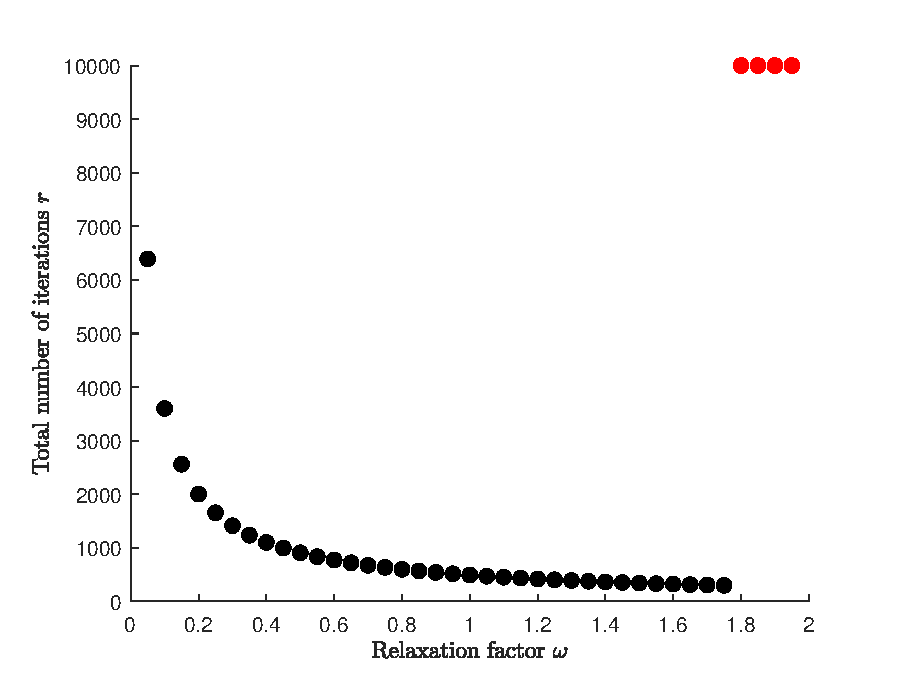
\includegraphics[width=7cm]{2-factor.eps}
        \caption{The figure shows the number of iterations of the sample case with $\varepsilon=10^{-6}$ for different relaxation factors. Red points indicate that the algorithm does not converge in $10^4$ iterations. They may converge in more iterations, but it is harmless to throw away these points.}
        \label{fig: q2}
    \end{figure}

    Fourth, we should verify that our algorithms do converge to the solution. As is shown in the outputs in \ref{appx: q2}, Frobenius norm of error of normal flux for each scheme is below $10^{-3}$.

    \section{Programs for Multigrid Routine}

    Outputs and codes are placed in \ref{appx: q3}.

    We have chosen the Galerkin prolongation and full weighting restriction operator in two dimensions described in the lecture note 7, and have applied an under-relaxed Jacobi smoother to code the generalized V-cycle multigrid routine as described in \ref{algo: V-cycle}. Remind that if the coarsest grid is set to be $2n$, then the generalized V-cycle multigrid routine will coincide with the two-grid method.

    \begin{algorithm}[htb]
        \caption{Generalized V-Cycle Multigrid Routine}
        \label{algo: V-cycle}

        \SetKwProg{Fn}{Function}{:}{end}
        \SetKwFunction{VCycle}{VCycleRecursive}

        \Fn{\VCycle{$u_n^r$, $f_n$}}{
            \KwIn{An initial guess matrix $u_n^r$ of the unknowns of size $(n+1)\times (n+1)$ and a force matrix $f_n$ of size $(n+1)\times (n+1)$}
            \KwOut{A new guess matrix $u^{r+1}$ of the unknowns of size $(n+1)\times (n+1)$}
            Relax $\upsilon_1$ times on $A_nu_n = f_n$ with initial guess $u_n^r$ and obtain $u_n^{r+1/3}$\;
            \If{$n$ is not the coarsest grid}{
                \For{$\upsilon_2$ times}{
                    Compute $r_n \leftarrow f_n - A_nu_n^{r+1/3}$ and restrict $r_n$ to obtain $r_{n/2}$\;
                    Solve $e_{n/2} \leftarrow \VCycle(0, r_{n/2})$\;
                    Prolongate $e_{n/2}$ to obtain $e_n$ and correct $u_n^{r+2/3}\leftarrow u_h^{r+1/3}+e_n$\;
                }
            }
            Relax $\upsilon_3$ times on $A_nu_n = f_n$ with intial guess $u_n^{r+2/3}$ and obtain $u_n^{r+1}$\;
        }
    \end{algorithm}

    No doubt that our algorithms converge to the solution. We have tested the efficiency of V-cycle routine with different parameters for the sample problem, and have found out that the 4 grid refinement V-cycle routine with relaxation factor $\omega=0.8$ and $\upsilon = (1, 1, 1)$ outperforms the others.

    \begin{table}[htb]
        \begin{center}
            \caption{We have applied V-cycle recursion scheme with different parameters to solve the problem of the sample problem for $\varepsilon=10^{-6}$ for 100 times in total, and have used \matlabinline{tic} and \matlabinline{toc} functions to measure the CPU time ellipsed in seconds. For comparison, note that Jacobi iteration scheme costs 1.022290 seconds while Gauss-Seidel iteration scheme with $\omega=1.75$ costs 0.284160 seconds.}
            \label{tbl: q3}
            \begin{tabular}{cccc}
                \toprule
                $\omega$ & max depth & $\upsilon$ & time ellipsed\\
                \midrule
                0.5 & 2 & (1, 2, 1) & 1.360112 \\
                0.8 & 2 & (1, 2, 1) & 0.889691 \\
                0.5 & 2 & (2, 4, 2) & 1.065023 \\
                0.8 & 2 & (2, 4, 2) & 0.696607 \\
                0.8 & 4 & (1, 2, 1) & 0.468962 \\
                0.8 & 4 & (1, 1, 1) & 0.160821 \\
                \bottomrule
            \end{tabular}
        \end{center}
    \end{table}

    \section{Programs and Solution for Anti-Problem}

    Outputs and codes are placed in \ref{appx: q4}.

    We apply 4 grid refinement V-cycle scheme with $\omega=0.8$ and $\upsilon=(1, 1, 1)$ to solve the anti-problem. It takes only 2.996252 seconds to iterate through $\binom{16}{4} = 1820$ cases, finding out that four source blocks are located at $(3, 5, 8, 15)$. See \ref{fig: q4-cfg} and \ref{fig: q4-exp}.

    \begin{figure}[htb]
        \centering
        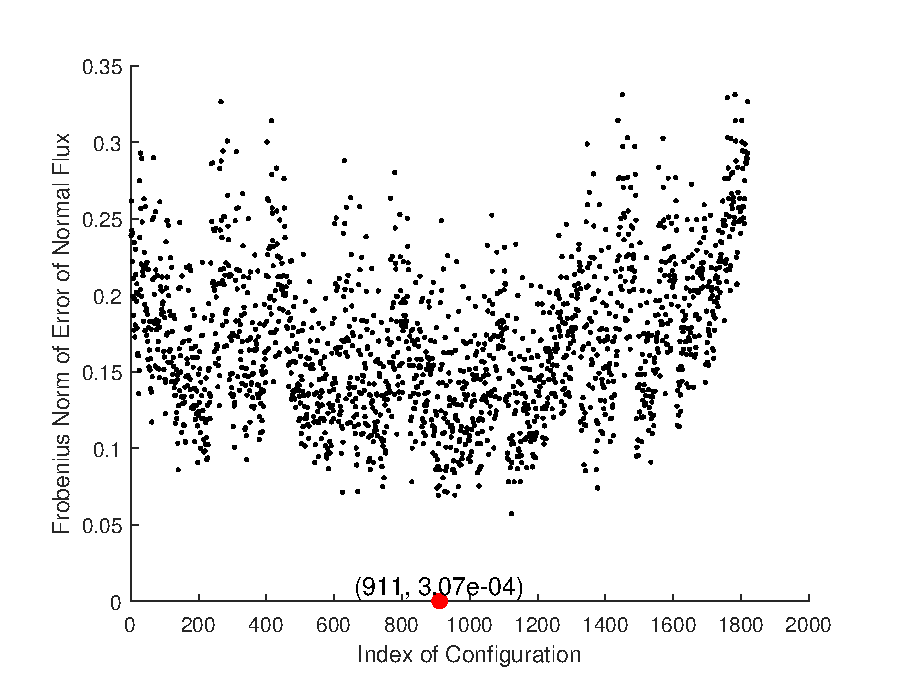
\includegraphics[width=7cm]{4-configuration.eps}
        \caption{The figure shows the Frobenius norms of errors of normal fluxes for different configurations of source blocks, where all configurations are generated by the MATLAB function \matlabinline{nchoosek}. The configuration of index 911 has much smaller error than any other configuration. Hence convincely, it is the solution we have been looking for.}
        \label{fig: q4-cfg}
    \end{figure}
    \begin{figure}[htb]
        \centering
        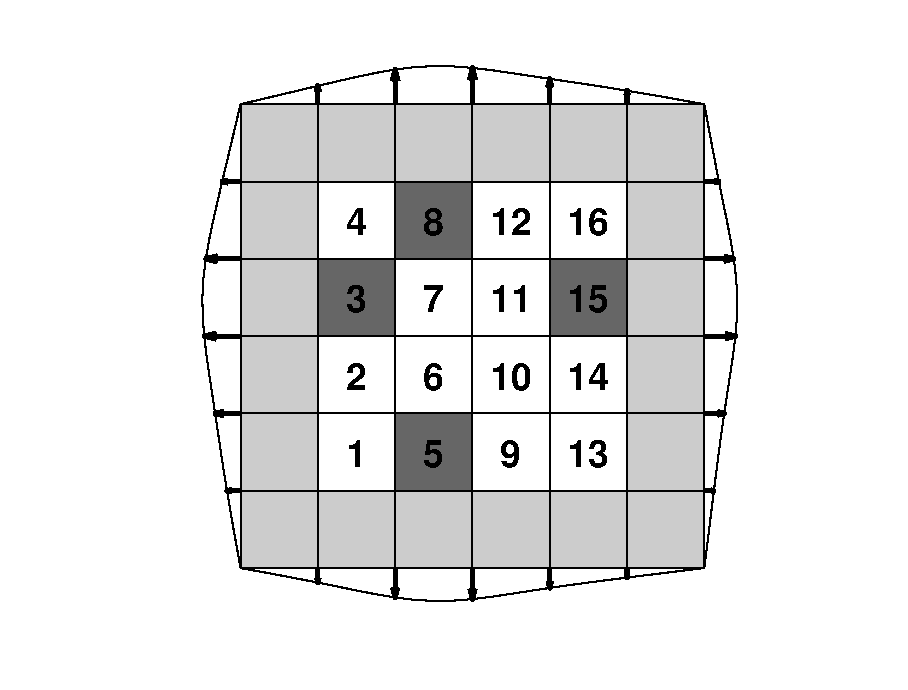
\includegraphics[width=7cm]{4-explanation.eps}
        \caption{The figure explains the solution of the anti-problem, where the dark blocks stand for source blocks, and the curve surrounding the unit square measures the normal flux at the boundary.}
        \label{fig: q4-exp}
    \end{figure}

    \clearpage
    \appendix
    \labelformat{section}{Appendix #1}

    The file structure of our MATLAB working folder is listed as follows, where those txt files store the values provided by the original problem with the first and last row being truncated.

    \begin{itemize}
        \item working\_folder
        \begin{itemize}
            \item compute\_flux.m
            \item edge\_zeros.m
            \item flux\_known.txt
            \item flux\_unknown.txt
            \item get\_F.m
            \item gs\_iteration\_matrix.m
            \item gs\_iteration.m
            \item jacobi\_iteration\_matrix.m
            \item jacobi\_iteration.m
            \item question\_2.m
            \item question\_3.m
            \item question\_4.m
            \item single\_jacobi\_iteration.m
            \item v\_cycle.m
        \end{itemize}
    \end{itemize}

    \section{Outputs and Codes for Jacobi and G-S Routines}\label{appx: q2}

    \begin{lstlisting}[style=MATLAB-editor, basicstyle=\ttfamily\scriptsize, title={Outputs}]
Jacobi iteration: 902 iterations in total; Frobenius norm of error is 3.9235e-04.
Gauss-Seidel iteration: 493 iterations in total; Frobenius norm of error is 3.2847e-04.
w: 0.05; iter: 6391; error: 2.24e-03.
w: 0.10; iter: 3601; error: 1.18e-03.
w: 0.15; iter: 2559; error: 8.34e-04.
w: 0.20; iter: 2003; error: 6.67e-04.
w: 0.25; iter: 1654; error: 5.71e-04.
w: 0.30; iter: 1414; error: 5.09e-04.
w: 0.35; iter: 1237; error: 4.67e-04.
w: 0.40; iter: 1102; error: 4.37e-04.
w: 0.45; iter: 995; error: 4.13e-04.
w: 0.50; iter: 907; error: 3.97e-04.
w: 0.55; iter: 835; error: 3.82e-04.
w: 0.60; iter: 773; error: 3.72e-04.
w: 0.65; iter: 721; error: 3.63e-04.
w: 0.70; iter: 675; error: 3.56e-04.
w: 0.75; iter: 635; error: 3.50e-04.
w: 0.80; iter: 600; error: 3.44e-04.
w: 0.85; iter: 569; error: 3.39e-04.
w: 0.90; iter: 541; error: 3.35e-04.
w: 0.95; iter: 516; error: 3.31e-04.
w: 1.00; iter: 493; error: 3.28e-04.
w: 1.05; iter: 472; error: 3.26e-04.
w: 1.10; iter: 453; error: 3.23e-04.
w: 1.15; iter: 435; error: 3.22e-04.
w: 1.20; iter: 419; error: 3.20e-04.
w: 1.25; iter: 404; error: 3.18e-04.
w: 1.30; iter: 390; error: 3.16e-04.
w: 1.35; iter: 377; error: 3.15e-04.
w: 1.40; iter: 365; error: 3.14e-04.
w: 1.45; iter: 354; error: 3.12e-04.
w: 1.50; iter: 343; error: 3.11e-04.
w: 1.55; iter: 333; error: 3.10e-04.
w: 1.60; iter: 324; error: 3.09e-04.
w: 1.65; iter: 315; error: 3.08e-04.
w: 1.70; iter: 307; error: 3.07e-04.
w: 1.75; iter: 299; error: 3.07e-04.
Warning: Algorithm has not converged in 1e4 iterations.
> In gs_iteration (line 38)
  In question_2 (line 28)
w: 1.80; iter: 10000; error: 3.39e-04.
Warning: Algorithm has not converged in 1e4 iterations.
> In gs_iteration (line 38)
  In question_2 (line 28)
w: 1.85; iter: 10000; error: 2.27e+01.
Warning: Algorithm has not converged in 1e4 iterations.
> In gs_iteration (line 38)
  In question_2 (line 28)
w: 1.90; iter: 10000; error: 4.29e+06.
Warning: Algorithm has not converged in 1e4 iterations.
> In gs_iteration (line 38)
  In question_2 (line 28)
w: 1.95; iter: 10000; error: 3.42e+14.
The optimal relaxation factor is 1.75.
    \end{lstlisting}

    \matlabinputlisting[caption={Function of Doing Stuff in one Iteration of Jacobi Iteration Scheme}]{single_jacobi_iteration.m}
    \matlabinputlisting[caption={Jacobi Iteration Scheme Using Double For-loops}]{jacobi_iteration.m}
    \matlabinputlisting[caption={Jacobi Iteration Scheme Using Matrix Translation}]{jacobi_iteration_matrix.m}
    \matlabinputlisting[caption={Gauss-Seidel Iteration Scheme Using Double For-loops}]{gs_iteration.m}
    \matlabinputlisting[caption={Gauss-Seidel Iteration Scheme Using Matrix Right Division}]{gs_iteration_matrix.m}
    \matlabinputlisting[caption={Function of Adding Zeros to the Edges of a Matrix}]{edge_zeros.m}
    \matlabinputlisting[caption={Function of Getting the Force Matrix of the Problem}]{get_F.m}
    \matlabinputlisting[caption={Main Script for Question 2}]{question_2.m}

    \section{Outputs and Codes for Multigrid Routine}\label{appx: q3}

    \begin{lstlisting}[style=MATLAB-editor, basicstyle=\ttfamily\scriptsize, title={Outputs}]
Jacobi: Elapsed time is 1.022290 seconds.
GS-1.75: Elapsed time is 0.284160 seconds.
VCycle-0.5-2-121: Elapsed time is 1.360112 seconds.
VCycle-0.8-2-121: Elapsed time is 0.889691 seconds.
VCycle-0.5-2-242: Elapsed time is 1.065023 seconds.
VCycle-0.8-2-242: Elapsed time is 0.696607 seconds.
VCycle-0.8-4-121: Elapsed time is 0.468962 seconds.
VCycle-0.8-4-111: Elapsed time is 0.160821 seconds.
    \end{lstlisting}

    \matlabinputlisting[caption={Generalized V-Cycle Multigrid Routine}]{v_cycle.m}
    \matlabinputlisting[caption={Main Script for Question 3}]{question_3.m}

    \section{Outputs and Codes for Anti-Problem}\label{appx: q4}

    \begin{lstlisting}[style=MATLAB-editor, basicstyle=\ttfamily\scriptsize, title={Outputs}]
Elapsed time is 2.996252 seconds.
    \end{lstlisting}

    \matlabinputlisting[caption={Main Script for Question 4}]{question_4.m}

\end{document}
